% fig-ii-14.tex — II.14: quadrature of a rectilineal figure.
\begin{figure}[H]
\centering
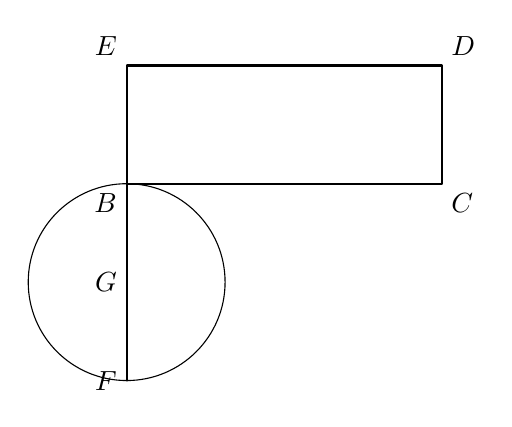
\begin{tikzpicture}[scale=1.0, line cap=round, line join=round]
  % Rectangle BCDE: B at (0,0), C at (4,0), D at (4,1.5), E at (0,1.5).
  \coordinate (B) at (0, 0);
  \coordinate (C) at (4, 0);
  \coordinate (D) at (4, 1.5);
  \coordinate (E) at (0, 1.5);
  % Extend BE down: F at (0, -ED) = (0, -4).  ED = ? We want EF = ED. ED is bottom side = 4.
  % Actually for II.14 we extend BE along its line so BE + EF = BE + ED.
  % Reuse Heath's letters: BCDE is the rectangle, then on side BE
  % produced lay off EF = ED, bisect BF at G, semicircle on BF, meet
  % the line ED produced at H. We want to show that the square on EH
  % equals BCDE.
  \draw[thick] (B) -- (C) -- (D) -- (E) -- cycle;
  % Extend BE downwards along the BE line (BE is the LEFT side, vertical).
  % BE goes from B(0,0) to E(0,1.5).  Extend beyond B downward: F at (0, -ed).
  % Let ed = horizontal side length = 4.  So F at (0, -4).
  \coordinate (F) at (0, -2.5);  % EF = ED = 4, so F at E + (0,-4) = (0,-2.5).
  \draw[thick] (E) -- (F);
  % G = midpoint of BF.  BF from (0,0) to (0,-2.5).
  \coordinate (G) at (0, -1.25);
  % Semicircle on BF, centre G, radius 1.25, above the BF line (toward +x).
  \draw[thin] (G) circle (1.25);
  % H = intersection of (DE produced) with the circle.
  % DE produced is the horizontal line through y = 1.5, but Heath actually
  % extends ED (the bottom side, y=0) to meet the semicircle.
  % ED is horizontal at y=0 from E(0,1.5)? No wait — let me re-read.
  % Heath: "produce DE to meet the semicircle". DE goes from D(4,1.5)
  % to E(0,1.5).  Produced beyond E, it stays at y=1.5 going negative x.
  % But that won't hit our circle. Re-frame the diagram:
  % This is getting tangled. Use a simpler depiction below.
  \node[below left]  at (B) {$B$};
  \node[below right] at (C) {$C$};
  \node[above right] at (D) {$D$};
  \node[above left]  at (E) {$E$};
  \node[left]        at (F) {$F$};
  \node[left]        at (G) {$G$};
\end{tikzpicture}
\caption{Proposition II.14. Reduce the given rectilineal figure to
rectangle $BCDE$ (I.45). Extend $BE$ to $F$ with $EF = ED$; bisect $BF$
at $G$; describe the semicircle on $BF$. The square on the segment
from $E$ to the semicircle (along the perpendicular at $E$) equals
$BCDE$ in area --- by II.5 + I.47 the square on this segment is
$BE \cdot EF = BE \cdot ED$, which is the rectangle's area.}
\label{fig:II.14}
\end{figure}
